\documentclass[twoside,10pt]{article}
\usepackage{shlists}
\usepackage[applemac]{inputenc}
\usepackage[spanish]{babel}
\usepackage[T1]{fontenc}


\usepackage{multicol}
\usepackage{picinpar}

\usepackage{url}
\newcommand{\surl}[1]{{\small\url{#1}}}

\newcounter{vol}
\newcounter{num}
\newcounter{anyo}
\setcounter{vol}{9}
\setcounter{num}{2}
\setcounter{anyo}{2016}
\newcommand{\mes}{Mayo}
\usepackage{revisionNLcol}


\title{\ \\ Docencia 2.0\\ \large Juan Juli\'{a}n Merelo, Fernando Tricas}
\author{\LARGE Lenguajes de programación: ¿uno, ninguno o todos?}

\date{}

\AutTit{Docencia 2.0}

\begin{document}
\addtocounter{page}{2}

\maketitle
\vspace*{-5ex}

\begin{multicols}{2}

Si hay un tema universal en la informática son los lenguajes de
programación. Desde los niveles más bajos de la arquitectura a los más
altos, la forma universal en la que el ser humano se comunica con un
ordenador son los programas, escritos en alguno de los lenguajes de
programación disponibles. Los lenguajes suelen tener una serie de
características comunes: una sintaxis rígida, implementaciones con
licencia libre y una evolución continua.
% No se muy bien a qué se refiere lo de implementaciones libres en este
% caso
% Implementaciones con licencia libre. Por ejemplo, el lenguaje-M de
% Matlab implementado con licencia libre es Octave.

En esta última característica está uno de los problemas. El lenguaje
que enseñaste en primero puede no parecerse en nada al que usarás en
el trabajo de fin de grado. Pero si consideramos que la evolución
individual está acompañada de una evolución colectiva de los tipos de
lenguajes que se usan y que, por tanto, se necesitan no ya para
conseguir un puesto de trabajo, sino siquiera para poder trabajar en
un entorno de computación determinado, la elección de un lenguaje de
programación para una asignatura o para una carrera entera se convierte en
una tarea ardua o imposible.

Porque, seamos prácticos, elegir un solo lenguaje para regirlos a
todos es imposible en nuestro país. Ni en ninguno, para el caso.
Nuestra idiosincrasia impediría que más de dos personas se pusieran de
acuerdo en qué lenguaje usar desde primero a cuarto, y en el caso
improbable de que un {\em ukase} de la superioridad impusiera uno, esa
misma idiosincrasia haría que el profesor de prácticas de 3º usara
eventualmente el que le viniera en gana. 
%Ahí va la mía
Seguramente esto es hasta sano y saludable porque, ¿quién nos aseguraría
que en el `mundo real' la sociedad y la industria habría elegido este
supuesto lenguaje ganador y tan perfecto para habernos puesto de acuerdo a
nosotros? Habrá que agradecerle al profesor de prácticas de 3º el que
el alumno  haya tenido exposición a diversos lenguajes y
entornos de trabajo, pero por esa misma razón descartada esa opción
del lenguaje único y puro para dominarlos a todos.

También podríamos pensar, siguiendo las metodologías modernas, la idea de
adaptación al estudiante: cada cuál que elija su lenguaje favorito y que lo
utilice
para desarrollar sus proyectos. Seguramente nos encontraríamos con algunas
dificultades: lenguajes poco adecuados para las tareas que están
relacionadas con la temática de la asignatura, excesivo `monocultivo',
dado que es fácil ponerse de acuerdo con uno mismo y terminar haciendo todo
con una sola tecnología, perdiendo la oportunidad de explorar otras, y la
no despreciable complejidad de prestar asistencia en caso de alguna cosa no
vaya bien. Desde nuestra experiencia esta puede ser una buena aproximación
cuando vamos avanzando en la carrera: Sugerir, por ejemplo, un lenguaje que
nosotros creamos adecuado pero facilitar que se elijan alternativas.
Eventualmente, el profesor no tiene que evaluar al
alumno por la letra de lo que haya hecho, es decir, la literalidad de
haber escrito algún algoritmo o usado una estructura de datos en un
lenguaje que el profesor conoce, sino por el hecho de que haya sido
capaz de entender esos conceptos y usarlos en la práctica. No
resultaría difícil, para cualquier profesor, evaluar la consecución de
los objetivos por parte del alumno en casi cualquier lenguaje de
programación. Salvo, quizá, Haskell. 

Vamos avanzando.

¿Y en primero? 
Lo que siempre se dice en estos casos es que se trata de aprender a
programar (sus bases, conceptos, la organización de un programa, entre
otros), y que el lenguaje no es lo
importante. Pero luego todo el mundo tiene argumentos para defender unos
y desdeñar otros.
%--------------------------
\noindent\rule{86mm}{1pt}
\vspace{1ex} {\small{\begin{window}[0,r,
\includegraphics[width = 27mm]{JJM.jpg},] 
\noindent\emph{JJ Merelo} es catedr\'{a}tico de Universidad
en el \'area de Arquitectura y Tecnolog\'{\i}a de Computadores, y
actualmente director de la Oficina de Software Libre de la UGR.
\'{U}ltimamente le ha dado por el \textsl{flipped
learning}, de lo que se informar\'{a} debidamente en esta columna.
\end{window}}}

\medskip

{\small{\begin{window}[0,r,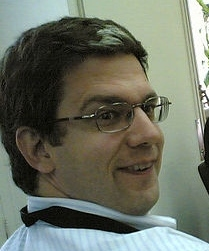
\includegraphics[width = 27 mm]{FTricas1.jpg},]
		\noindent \emph{Fernando Tricas Garc\'{\i}a} es profesor
		titular de Lenguajes y Sistemas Inform\'{a}ticos del Departamento
		de Inform\'{a}tica e Ingenier\'{\i}a de Sistemas de la Universidad de
		Zaragoza.  Empez\'{o} a estudiar la blogosfera casi cuando a\'{u}n no
		exist\'{\i}a (all\'{a} por el a\~{n}o 2002) y a tratar de integrarla en los
		cursos y tareas docentes un poco despu\'{e}s.  Ha impartido
		numerosas charlas relacionadas con el tema de la Web 2.0, 

		internet y universidad,\ldots\ 
		Es actualmente Vicerrector de Tecnolog\'{\i}as de la Informaci\'{o}n y
de la Comunicaci\'{o}n.   
		\end{window}}}
%-------------------------------------------------

El problema es que, frente a la posibilidad de que el alumno use su
propio lenguaje o tener un sólo lenguaje, nos barruntamos que obligar
al alumno de primero a usar varios lenguajes, diferentes, cada uno con
sus bases, su historia, sus herramientas, es la peor opción. Realmente
no hay lenguaje de programación moderno, sí, hasta PHP, que no
implemente todos los conceptos que debe aprender un alumno de
primero. El adoptar un sólo lenguaje permitiría a los profesores
concentrarse en los conceptos en sí, y no tener que dedicar una o
varias sesiones de prácticas a las complejidades intrínsecas de
compilar en Java o en Pascal o cómo instalar paquetes en R. Una
encuesta informal en cualquier escuela de informática te permitirá
descubrir que en primero, y muchas veces en el primer cuatrimestre,
diferentes asignaturas usan lenguajes o entornos tan disimilares como
R, Maxima, Java, C++, Python e incluso C puro y duro, además de algún
que otro lenguaje máquina. Todo ello en primero de carrera, en los
primeros meses, y en aras de {\em facilitar al alumno la tarea}. 

Nada más lejos de la realidad. El principal obstáculo para la
implantación de Un Solo Lenguaje en primero es la imposibilidad
% Esas mayúsculas? Un Solo Lenguaje?
práctica de que una serie de profesores de diferentes departamentos,
procedencias y talantes se pongan de acuerdo y/o sean capaces de
aprender un nuevo lenguaje de programación. Lo que se le exige al
alumno, aprender varios lenguajes en lo que dura un cuatrimestre, es
algo que el profesor es incapaz de hacer en los trienios y sexenios
que tiene acreditados como docente. Todo ello redunda en las altísimas
tasas de abandono de la carrera, de las más altas entre las
ingenierías. 
% Veo este párrafo demasiado duro...

Imaginad que los alumnos llegaran a 2º controlando bien, con cierta
eficacia, un lenguaje, uno solo. Eso permitiría, a partir de ahí,
dejarle libertad para que elija nuevos lenguajes en asignaturas, como
las que se dan en segundo, que no están especializadas en un lenguaje
específico. Usando como base, por supuesto, ese lenguaje que se conoce
en primero. La situación actual lo que hace es que, llegado 2º, los
alumnos han olvidado casi totalmente los lenguajes usados en
asignaturas de físicas y matemáticas, olvidado también C y C++ si es
que no se continúa con ellos, y haber aprendido un poco de Java, que
quizás tengan que olvidar más adelante si empiezan a usar lenguajes de
scripting como Python o PHP en asignaturas relacionadas con la
web. ¿Cuantas horas de experiencia tiene el alumno graduado en un
lenguaje determinado? Demasiadas pocas.
% Y este demasiadas generalizaciones.
% De hecho, creo que es saludable que lleguen a segundo habiendo utilizado
% varios lenguajes porque eso les permite extraer sus propias
% generalizaciones (lo que todos tienen, en qué cosas son diferentes,...),
% aunque no los dominen todos. De hecho, quiero creer que en la mayoría de
% las titulaciones tendrán un lenguaje más o menos instrumental para las
% asignaturas de programación y además hayan visto el c o el ensamblador
% con los de sistemas operativos, arquitectura o lo que sea y el que se les
% haya ocurrido a los de matemáticas que habrán elegido el que
% se les haya ocurrido. Pero yo lo veo positivo, en general.
% Por otro lado, escribir todo tan negativo va a hacer que la gente se fije
% en la parte negativa y no tanto en el mensaje, no se.

Pensemos, pues, en las bondades de la Gran Unificación de Lenguajes en
la carrera de informática. Aunque los méritos de cada lenguaje
específico es algo que dejaremos para una columna próximamente. 

\noindent  
\bigskip

\noindent\emph{Todas las columnas de la serie Docencia 2.0
pueden descargarse en formato LaTeX desde
\surl{https://github.com/ReVision-Docencia-20/Columnas}}

\noindent\rule{90mm}{1pt}

{\small \noindent\copyright 2016 JJ. Merelo, F. Tricas. Este art\'{\i}culo es de acceso libre distribuido bajo los t\'{e}rminos
de la Licencia Creative Commons de Atribuci\'{o}n, que permite copiar,
distribuir y comunicar p\'{u}blicamente la obra en cualquier medio, s\'{o}lido
o electr\'{o}nico, siempre que se acrediten a los autores y fuentes
originales}

\end{multicols}
\end{document}
